\documentclass{report}
\title{Proposition de th\`ese}
\author{Yannick Hold-Geoffroy  \\
    Universit\'e laval  \\
    }

\date{\today}


\usepackage[utf8]{inputenc}
\usepackage{times}
\usepackage{amsmath}
\usepackage{amssymb}
\usepackage{cite}   % sort citation numbers automatically
\usepackage{url}
\usepackage{graphicx}
\usepackage{rotating}
%\usepackage{authblk}
% to control spacing in item lists
\usepackage{enumitem}
\usepackage[pagebackref=false,breaklinks=true,colorlinks,bookmarks=false]{hyperref}


% Hint: \title{what ever}, \author{who care} and \date{when ever} could stand 
% before or after the \begin{document} command 
% BUT the \maketitle command MUST come AFTER the \begin{document} command! 
\begin{document} 

\maketitle

\tableofcontents

% Commands
\newcommand{\boldomega}{\boldsymbol \omega} % bold omega
\newcommand{\boldmu}{\boldsymbol \mu} % bold omega
\newcommand{\bolddelta}{\boldsymbol \delta} % bold delta

\graphicspath{{figures/}}

%\begin{abstract}
%\end{abstract}


\chapter*{Symboles et notations}

\begin{table}[htbp]\caption{Symboles et notations}
\centering % to have the caption near the table
\begin{tabular}{r c p{10cm} }

\hline & & \\
$\langle \cdot, \cdot \rangle$      & $=$ & Produit scalaire \\
$\bold{x}$                          & $=$ & Vecteur \\
$X$                                 & $=$ & Matrice \\
$\omega$                            & $=$ & Angle \\
\hline
\end{tabular}
\label{tab:TableOfNotationForMyResearch}
\end{table}


%%%%%%%%%%%%%%%%%%%%%%%%%%%%%%%%%%%%%%%%%%%%%%%%%%%%%%%%%%%%%%%%%%%%%%%%%%%%%%%%
\chapter{Introduction}

%Comment la numérisation du monde est à nos portes et c'est le futur.
%La reconstruction 3d est un sujet de plus en plus présent dans la vie de tous les jours.

%Reconstruction 3D extérieure à large échelle.

%Utilisations: Jeux vidéos, préserver la culture, réalité augmentée, diffusion


\section{Stéréoscopie Photométrique}

Décrire la PS, ses entrées, ses sorties, ses forces (1 normale par px), ses faiblesses, citer Woodham.

%La Stéréoscopie Photométrique (SP) est une technique permettant de récupérer la structure d'une scène à partir d'indices photométriques. Elle donne en sortie une carte de normale. Cette carte définie, pour chaque pixel de l'image, la normale de la surface correspondante dans la scène. Une fois la carte de normale obtenue, il est possible de l'intégrer afin d'obtenir un maillage 3d de la surface.

%Pour fonctionner, la PS a besoin d'une séquence d'images en entrée.

\section{Stéréoscopie Photométrique}

Dans sa forme de base, la SP...

\cite{Woodham1979}

\begin{equation}
\bold{b} = \rho L(\mathbf{\boldomega}) \langle \boldomega, {\bf n} \rangle \,,
\end{equation}

\begin{figure}
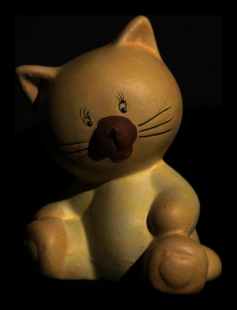
\includegraphics[width=.1\linewidth]{PS/cat_0.png}
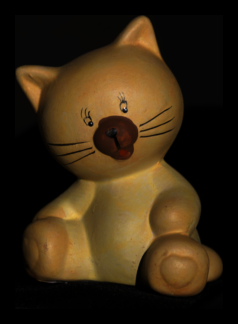
\includegraphics[width=.1\linewidth]{PS/cat_1.png}
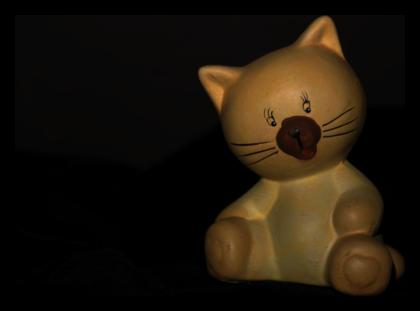
\includegraphics[width=.1\linewidth]{PS/cat_2.png}
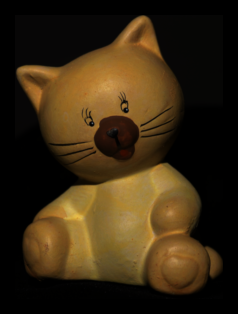
\includegraphics[width=.1\linewidth]{PS/cat_3.png}
\caption{Exemples d'images d'entrée}
\label{fig:fig}
\end{figure}


PS was confined to the lab until recently.

Illumination incontrôlable, coplanarité du soleil.


%%%%%%%%%%%%%%%%%%%%%%%%%%%%%%%%%%%%%%%%%%%%%%%%%%%%%%%%%%%%%%%%%%%%%%%%%%%%%%%%
\chapter{Revue de littérature}

Expliquer les améliorations de la PS au travers du temps:
\begin{itemize}
	\item Unknown lighting
	\item Unknown BRDF
	\item Robustness
	\item Outdoor (algorithme et analyse)
	\begin{itemize}
		\item Yu
		\item Boxin shi
	\end{itemize}
\end{itemize}

%\cite{Hold-Geoffroy-3DV15,Hold-Geoffroy-ICCP15}


%%%%%%%%%%%%%%%%%%%%%%%%%%%%%%%%%%%%%%%%%%%%%%%%%%%%%%%%%%%%%%%%%%%%%%%%%%%%%%%%
\chapter{Existing contributions}


\section{}
ICCP15

\section{}
3DV15


%%%%%%%%%%%%%%%%%%%%%%%%%%%%%%%%%%%%%%%%%%%%%%%%%%%%%%%%%%%%%%%%%%%%%%%%%%%%%%%%
\chapter{Proposed contributions}

\section{Modèles d'illumination plus riche ( Already done, put it 1) Introduction (In this thesis...), 2) ensure it's in the previous work )}

Décrire le Mean Light Vector, décrire notre base de données de ciels, décrire comment on peut appliquer la philosophie Big Data à ce problème.

\begin{equation}
b_t = \frac{\rho}{\pi} \int_{\Omega_{\bf n}} L_t(\mathbf{\boldomega}) \langle \boldomega, {\bf n} \rangle d\omega \,,
\end{equation}

\section{Calibrated outdoor reconstruction}

\section{Blind outdoor reconstruction}

\section{Emploi d'autres astres que le soleil}

Décrire le projet day \& night.

\section{Augmentation avec d'autres techniques}

Décrire l'amélioration que pourrait apporter la PS utilisée conjointement avec du SFM et la stéréo multivues standard.


%%%%%%%%%%%%%%%%%%%%%%%%%%%%%%%%%%%%%%%%%%%%%%%%%%%%%%%%%%%%%%%%%%%%%%%%%%%%%%%%
\chapter{Échéancier}

\begin{itemize}
	\item 2016h: Selection and Calibrated PS algorithm
	\item 2016e: Capture, Blind PS algorithm  
	\item 2016a: Blind PS algorithm, Day \& night
	\item 2017h: Fusion with SFM
	\item 2017e: Capture, Fusion with Multiview Stereo Techniques
	\item 2017a: 
	\item 2018h: Écrire et soutenir.
\end{itemize}


%%%%%%%%%%%%%%%%%%%%%%%%%%%%%%%%%%%%%%%%%%%%%%%%%%%%%%%%%%%%%%%%%%%%%%%%%%%%%%%%
\chapter{Conclusion}\label{conclusion}

Recap.

{\small
%\bibliographystyle{ieee}
\bibliography{main}
}

\end{document}
